\documentclass[10pt]{beamer}
\usepackage[utf8]{inputenc}
\usepackage[main=vietnamese, english]{babel}
\usepackage[T1]{fontenc}
\usepackage{multicol}
\usepackage{color}
\setlength{\columnseprule}{1pt}
\def\columnseprulecolor{\color{blue}}
\usepackage{lmodern}
\usetheme{CambridgeUS}
\title{\textbf{Các mô hình ngẫu nhiên và ứng dụng}}

\author[Nhóm  thực hiện: 22]{\textbf{\fontsize{14pt}{17pt}{Giảng viên hướng dẫn: TS Nguyễn Thị Ngọc Anh\\Viện Toán ứng dụng và Tin học}}}
\institute[]{
	\includegraphics[scale=.3]{hinh1}}
\date[15/07/2020]{Thứ tư, ngày 15 tháng 07 năm 2020}
\begin{document}
	%\author{}
	%\title{}
	%\subtitle{}
	%\logo{}
	%\institute{}
	%\date{}
	%\subject{}
	%\setbeamercovered{transparent}
	%\setbeamertemplate{navigation symbols}{}
	\begin{frame}[plain]
	\maketitle
\end{frame}

\begin{frame}
\frametitle{Danh sách thành viên}
	\begin{center}
		\begin{tabular}{|l|c|l|}
			\hline
			\color{blue}{\textbf{Họ và tên}} & \color{blue}{\textbf{MSSV}} & \color{blue}{\textbf{Phân công}}\\ \hline
			
			\textbf{Nguyễn Thiện Đông} & 20161027 & Viết báo cáo + Demo Code \\ \hline
			\textbf{Ngô Gia Lâm} & 20162311 & Tìm tài liệu + Báo cáo\\ \hline
			\textbf{Nguyễn Bá Kiên} & 20152057 & Tìm tài liệu + Báo cáo\\ \hline
		\end{tabular}
	\end{center}	
\end{frame}

\begin{frame}
\frametitle{Nội dung}
	\tableofcontents
\end{frame}
%%%%%%%%%%%%%%%%%%%%%%%%%%%%%%%%%%%%%%%%%%%%%%%%%%%%%%%%%%%%%%%%%%%%%%%%%%%%%%%%%%%%%%%%%%%%%%%%%%%%%%%
\section{Lý thuyết hàng đợi}
\begin{frame}
	\frametitle{Lý thuyết hàng đợi}
\end{frame}
%%%%%%%%%%%%%%%%%%%%%%%%%%%%%%%%%%%%%%%%%%%%%%%%%%%%%%%%%%%%%%%%%%%%%%%%%%%%%%%%%%%%%%%%%%%%%%%%%%%%%%%
\subsection{Giới thiệu chung}
\begin{frame}
\frametitle{Lý thuyết hàng đợi}
\begin{block}{\textbf{Giới thiệu chung}}
	Lý thuyết xếp hàng là một trong các công cụ toán học mạnh mẽ cho việc phân tích, ước lượng trong các hệ thống hàng đợi. Lý thuyết xếp hàng thông thường được áp dụng cho các hệ thống lý tưởng để đưa ra các kết quả gần đúng cho một mô hình thực tế. Tính chất chung của các giải pháp ứng dụng lý thuyết xếp hàng là làm rõ lưu lượng dòng vào, để cung cấp dự báo nhứng danh giới lớn hơn trên những kết quả nghiên cứu thu được. Chúng rất hữu ích cho việc xác định tính đúng đắn của các phương pháp.

\end{block}
\end{frame}
%%%%%%%%%%%%%%%%%%%%%%%%%%%%%%%%%%%%%%%%%%%%%%%%%%%%%%%%%%%%%%%%%%%%%%%%%%%%%%%%%%%%%%%%%%%%%%%%%%%%%%%
\subsection{Định nghĩa}
\begin{frame}
\frametitle{Lý thuyết hàng đợi}
\begin{block}{\textbf{Định nghĩa}}
\par Một quá trình xếp hàng là:
\begin{itemize}
    \item Dòng khách hàng tới
    \item Khả năng phục vụ của server
    \item Nếu khách hàng tới chưa được phục vụ thì sẽ xếp xếp hàng
    \item Hệ thống xếp hàng gồm khách hàng trong hàng đợi và khách hàng đang được phục vụ.
\end{itemize}
\end{block}
\end{frame}
%%%%%%%%%%%%%%%%%%%%%%%%%%%%%%%%%%%%%%%%%%%%%%%%%%%%%%%%%%%%%%%%%%%%%%%%%%%%%%%%%%%%%%%%%%%%%%%%%%%%%%%
\begin{frame}
\frametitle{Lý thuyết hàng đợi}
\begin{block}
\par Chuẩn ký hiệu cho hệ thống xếp hàng được sắp xếp như sau:\\
Dòng vào / dòng phục vụ / số lượng server / số lượng khách hàng lớn nhất trong hệ thống / quy tắc xếp hàng.
\begin{itemize}
    \item Dòng vào: lượng khách tới hệ thống
    \item Dòng phục vụ: lượng khách được phục vụ xong ra khỏi server
    \item Số server: số kênh phục vụ
    \item  Lượng khách lớn nhất: tổng lượng khách đang phục vụ và trong xếp hàng
    \item Quy tắc xếp hàng: Một số nguyên tắc phục vụ thường được áp dụng trong các hệ thống hàng đợi là FIFO (First in first out), LIFO (Last in first out), FCFS (First come first serve), có ưu tiên, không ưu tiên, Random Order...
\end{itemize}
\end{block}
\end{frame}
%%%%%%%%%%%%%%%%%%%%%%%%%%%%%%%%%%%%%%%%%%%%%%%%%%%%%%%%%%%%%%%%%%%%%%%%%%%%%%%%%%%%%%%%%%%%%%%%%%%%%%%
\subsection{Các phương pháp giải bài toán mô hình xếp hàng}
\begin{frame}
\frametitle{Lý thuyết hàng đợi}
\begin{block}{\textbf{Các phương pháp giải bài toán mô hình xếp hàng}}
\begin{minipage}{5.5cm}
\begin{block}
    \par Phương pháp giải tích\\
    \begin{itemize}
        \item B1: Phân tích hệ thống
        \item B2: Thiết lập hệ phương trình trạng thái cho các xác suất trạng thái
        \item B3: Giải hệ tìm các xác suất trạng thái
        \item B4: Tính toán phân tích các chỉ tiêu đưa ra nhận xét và quyết định
    \end{itemize}
\end{block}
\end{minipage}
\hfill
\begin{minipage}{5.5cm}
\begin{block}
    \par Phương pháp mô phỏng trên máy tính
    \begin{itemize}
        \item B1: Xác định bài toán
        \item B2: Đo và thu thập dữ liệu cần thiết để khảo sát
        \item B3: Chạy mô phỏng kiểm chứng, so sánh thực tế. Phân tích kết quả nếu cần thì sửa lại phương án được đánh giá qua mô phỏng 
        \item B4: Triển khai thực tế
    \end{itemize}
\end{block}
\end{minipage}
\end{block}
\end{frame}
%%%%%%%%%%%%%%%%%%%%%%%%%%%%%%%%%%%%%%%%%%%%%%%%%%%%%%%%%%%%%%%%%%%%%%%%%%%%%%%%%%%%%%%%%%%%%%%%%%%%%%%
\subsection{Các yếu tố cơ bản của hệ thống xếp hàng}
\begin{frame}
\frametitle{Lý thuyết hàng đợi}
\begin{block}{\textbf{Các yếu tố cơ bản của hệ thống xếp hàng}}
\begin{center}
    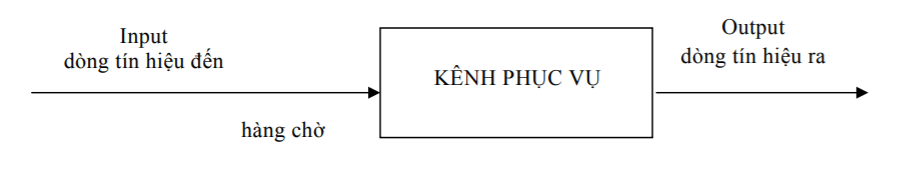
\includegraphics[scale=.5]{img/HeThongHangCho.PNG}
\end{center}
Bố trí vật lý:
\begin{center}
    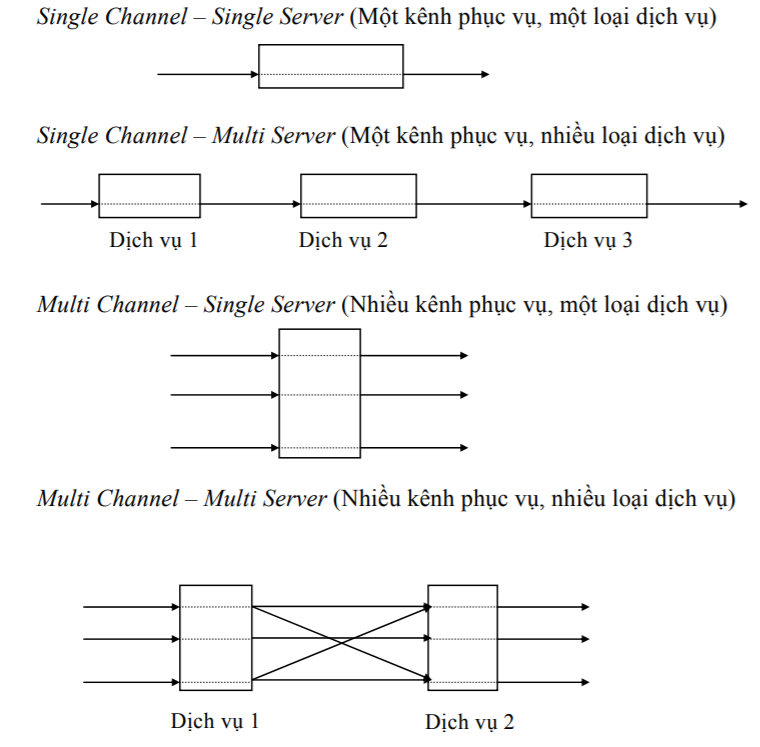
\includegraphics[scale=.5]{img/CacDangHTHangCho.PNG}
\end{center}
\end{block}
\end{frame}
%%%%%%%%%%%%%%%%%%%%%%%%%%%%%%%%%%%%%%%%%%%%%%%%%%%%%%%%%%%%%%%%%%%%%%%%%%%%%%%%%%%%%%%%%%%%%%%
\begin{frame}
\frametitle{Lý thuyết hàng đợi}
\begin{block}{\textbf{Các yếu tố cơ bản của hệ thống xếp hàng}}
\par Nguyên tắc phục vụ:
\begin{itemize}
    \item FIFO (First In First Out)
    \item LIFO (Last in first out)
    \item FCFS(First come first serve)
    \item Có ưu tiên
    \item Không ưu tiên
\end{itemize}
\end{block}
\end{frame}
%%%%%%%%%%%%%%%%%%%%%%%%%%%%%%%%%%%%%%%%%%%%%%%%%%%%%%%%%%%%%%%%%%%%%%%%%%%%%%%%%%%%%%%%%%%%%%%
\subsection{Một số điểm hạn chế của hệ thống xếp hàng}
\begin{frame}
\frametitle{Lý thuyết hàng đợi}
\begin{block}{\textbf{Một số điểm hạn chế của hệ thống xếp hàng}}
Các mô hình xếp hàng giới thiệu ở trên là những mô hình tiện lợi nhất
được áp dụng khá rộng rãi. Tuy nhiên, do các mô hình này công nhận các
giả thuyết \textit{quá chặt chẽ} ít xảy ra trên thực tế, nên các chuyên gia trong
lĩnh vưc Toán ứng dụng/Khoa học quản lí cũng đã đề xuất
xem xét nhiều mô hình khác như: số
tín hiệu cần phục vụ là hữu hạn, dòng tín hiệu đến là Poisson, cường độ
phục vụ phụ thuộc vào số tín hiệu trong xếp hàng ... \\
Trong thực tiễn, các hệ thống xếp hàng không bao giờ đạt
tới trạng thái vững. Chẳng hạn, trong một hệ thống xếp hàng, cường
độ tín hiệu đến trung bình thay đổi nhiều lần trong ngày không cho phép
hệ thống đạt được trạng thái vững.
Do đó, để giải quyết cần áp dụng phương pháp mô phỏng để tìm ra lời giải có tính thực tiễn cho các mô hình xếp hàng khi hệ thống
không thể đạt tới trạng thái vững hoặc khi không có các mô hình lí thuyết
thích hợp.
\end{block}
\end{frame}
%%%%%%%%%%%%%%%%%%%%%%%%%%%%%%%%%%%%%%%%%%%%%%%%%%%%%%%%%%%%%%%%%%%%%%%%%%%%%%%%%%%%%%%%%%%%%%%
\subsection{Ứng dụng}
\begin{frame}
\frametitle{Lý thuyết hàng đợi}
\begin{block}{\textbf{Ứng dụng}}
\begin{itemize}
    \item Áp dụng cho bài toán bán vé
    \item Viễn thông
    \item Điều khiển giao thông
    \item Xác định trình tự của hệ thống máy tính
    \item Dự báo hiệu suất của máy tinh
    \item Dịch vụ sức khỏe
\end{itemize}
\end{block}
\end{frame}
%%%%%%%%%%%%%%%%%%%%%%%%%%%%%%%%%%%%%%%%%%%%%%%%%%%%%%%%%%%%%%%%%%%%%%%%%%%%%%%%%%%%%%%%%%%%%%%
\section{Áp dụng cho bài toán bán vé}
\begin{frame}
	\frametitle{Áp dụng cho bài toán bán vé}
\end{frame}
\subsection{Đề bài}
\begin{frame}
	\frametitle{Áp dụng cho bài toán bán vé}
	\begin{block}{\textbf{Đề bài}}
	Giả sử dòng khách hàng tới mua vé tại một ga tàu với M quầy phục vụ là dòng Poisson	với tham số $\lambda$ là số khách hàng /1 phút, ví dụ $\lambda = 6$ (có nghĩa là khách hàng đến phòng bán vé với các thời điểm tuân theo luật phân phối mũ với tham số $\lambda = 6$). Ngoài ra, còn biết nguyên tắc phục vụ là FCFS (First come first serve) và thời gian phục vụ tại mỗi quầy có luật phân phối mũ với kì vọng $t$ (phút). Suy ra, $\mu = \frac{1}{t}$ 
	\end{block}	
\end{frame}
%%%%%%%%%%%%%%%%%%%%%%%%%%%%%%%%%%%%%%%%%%%%%%%%%%%%%%%%%%%%%

%%%%%%%%%%%%%%%%%%%%%%%%%%%%%%%%%%%%%%%%%%%%%%%%%%%%%%%%%%%
\subsection{Hệ thống hàng đợi M/M/C/K}
\begin{frame}
	\frametitle{Áp dụng cho bài toán bán vé}
	\begin{block}{\textbf{Hệ thống hàng đợi M/M/C/K}}
\begin{itemize}
    \item Có tiến trình đến là một tiến trình phân phối Poisson
    \item Hệ thống phục vụ có thời gian dịch vụ là một biến ngẫu nhiên phân phối mũ.
    \item C là số trạm phục vụ (server) khách hàng
    \item K là số lượng khách có thể chứa tối đa trong hệ thống .
\end{itemize}	
\end{block}
\end{frame}
%%%%%%%%%%%%%%%%%%%%%%%%%%%%%%%%%%%%%%%%%%%%%%%%%%%%%%%%%%%%
\begin{frame}
\frametitle{Áp dụng cho bài toán bán vé}
\begin{block}{\textbf{Hệ thống hàng đợi M/M/C/K}}
	\begin{center}
		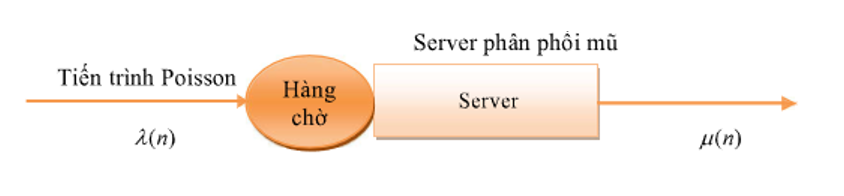
\includegraphics[scale=.8]{img/HT_MMCK.PNG}
	\end{center}
	\begin{center}
		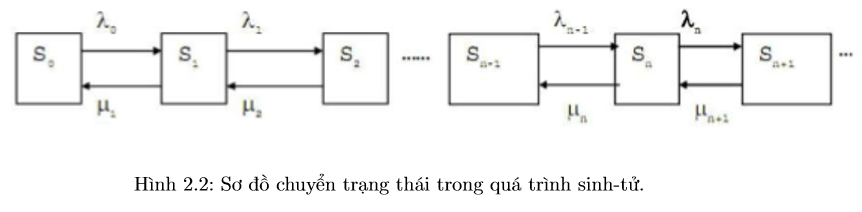
\includegraphics[scale=.8]{img/QT_SinhTu.PNG}
	\end{center}
\end{block}
		
\end{frame}
%%%%%%%%%%%%%%%%%%%%%%%%%%%%%%%%%%%%%%%%%%%%%%%%%%%%%%%%%%%%

\subsection{Giải quyết bài toán}
\begin{frame}
	\frametitle{Áp dụng cho bài toán bán vé}
	\begin{block}{\textbf{Giải quyết bài toán}}
    \par Bài toán có $K+1$ trạng thái:
    $\lambda_i = \lambda, \forall i = 1,...,n$
    \begin{align*} \mu_n =
        \begin{cases}
        n \mu , n = 1,...,c-1\\
        c \mu , n = c,c+1,...
        \end{cases}
    \end{align*}
 \par Thiết lập ma trận sinh theo công thức:
    \begin{align*} G=
    \begin{bmatrix}
        -\lambda_0 & \lambda_0 \\
        \mu_1 & -(\mu_1 + \lambda_1) & \lambda_1\\
        &\mu_2 & -(\mu_2 + \lambda_2) & \lambda_2\\
        & & {\boldsymbol{\ddots}} & {\boldsymbol{\ddots}} &{\boldsymbol{\ddots}}\\
        & & & & & \lambda_n\\
        & & & &  \mu_n & -\mu_n
    \end{bmatrix}
\end{align*}
\end{block}
\end{frame}
%%%%%%%%%%%%%%%%%%%%%%%%%%%%%%%%%%%%%%%%%%%%%%%%%%%%%%%%%%%%
\begin{frame}
	\frametitle{Áp dụng cho bài toán bán vé}
	\begin{block}
\par Phân phối dừng của lượng người trong hệ thống bán vé là vectơ $\pi$ là nghiệm của hệ
\begin{align*}
    \begin{cases}
    \pi G = 0 \\
    \displaystyle\sum_{i=0}^{k+1} \pi_i = 1
    \end{cases}
\end{align*}
Từ đó ta suy ra được phân phối dừng của hệ thống\\
\end{block}
\end{frame}
%%%%%%%%%%%%%%%%%%%%%%%%%%%%%%%%%%%%%%%%%%%%%%%%%%%%%%%%%%%%%%%%%
\begin{frame}
	\frametitle{Áp dụng cho bài toán bán vé}
	\begin{block}{Các đại lượng của mô hình M/M/1/K}
\begin{center}
    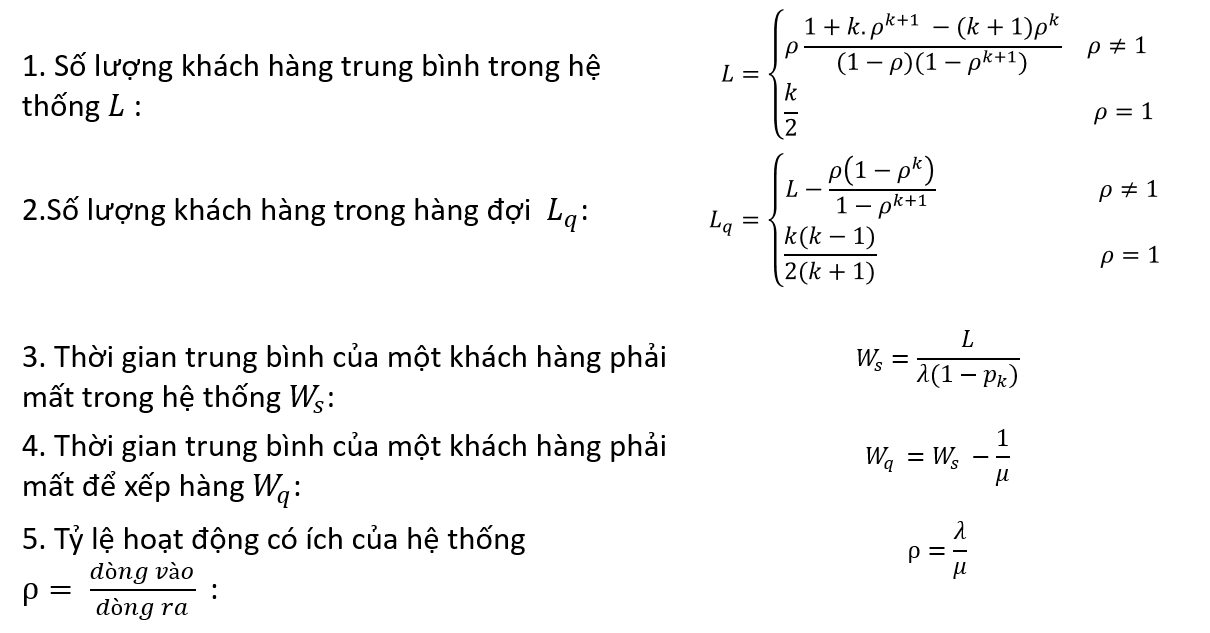
\includegraphics[scale=.5]{img/MM1k.PNG}
\end{center}

\end{block}
\end{frame}
%%%%%%%%%%%%%%%%%%%%%%%%%%%%%%%%%%%%%%%%%%%%%%%%%%%%%%%%%%%%%%%%%
\begin{frame}
	\frametitle{Áp dụng cho bài toán bán vé}
	\begin{block}{Các đại lượng của mô hình M/M/1/K}
\begin{center}
    \includegraphics[scale=.5]{img/MM1k.2.PNG}
\end{center}

\end{block}
\end{frame}
%%%%%%%%%%%%%%%%%%%%%%%%%%%%%%%%%%%%%%%%%%%%%%%%%%%%%%%%%%%%%%%%%
\begin{frame}
	\frametitle{Áp dụng cho bài toán bán vé}
	\begin{block}{Các đại lượng của mô hình M/M/C/K}
\begin{center}
    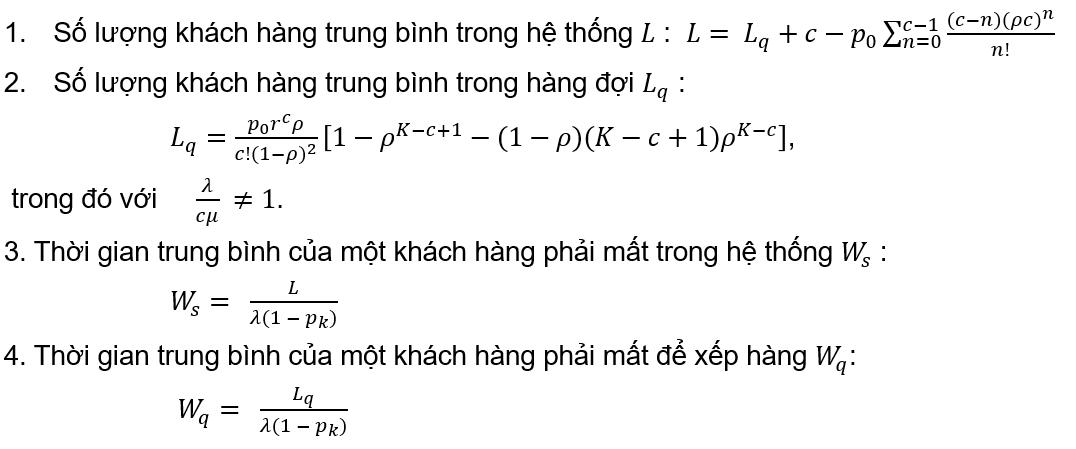
\includegraphics[scale=.5]{img/mmck.1.PNG}
\end{center}

\end{block}
\end{frame}
%%%%%%%%%%%%%%%%%%%%%%%%%%%%%%%%%%%%%%%%%%%%%%%%%%%%%%%%%%%%%%%%%
\begin{frame}
	\frametitle{Áp dụng cho bài toán bán vé}
	\begin{block}{Các đại lượng của mô hình M/M/C/K}
\begin{center}
    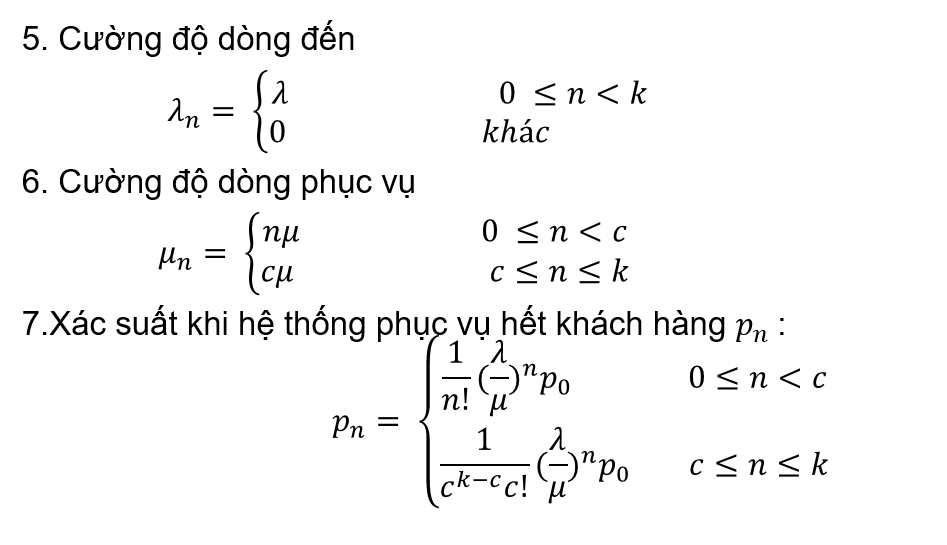
\includegraphics[scale=.5]{img/mmck.2.PNG}
\end{center}

\end{block}
\end{frame}
%%%%%%%%%%%%%%%%%%%%%%%%%%%%%%%%%%%%%%%%%%%%%%%%%%%%%%%%%%%%%%%%%
\subsection{Chương trình}
\begin{frame}
	\frametitle{Áp dụng cho bài toán bán vé}
	\begin{block}{\textbf{Chương trình}}
	\begin{center}
    \begin{center}
     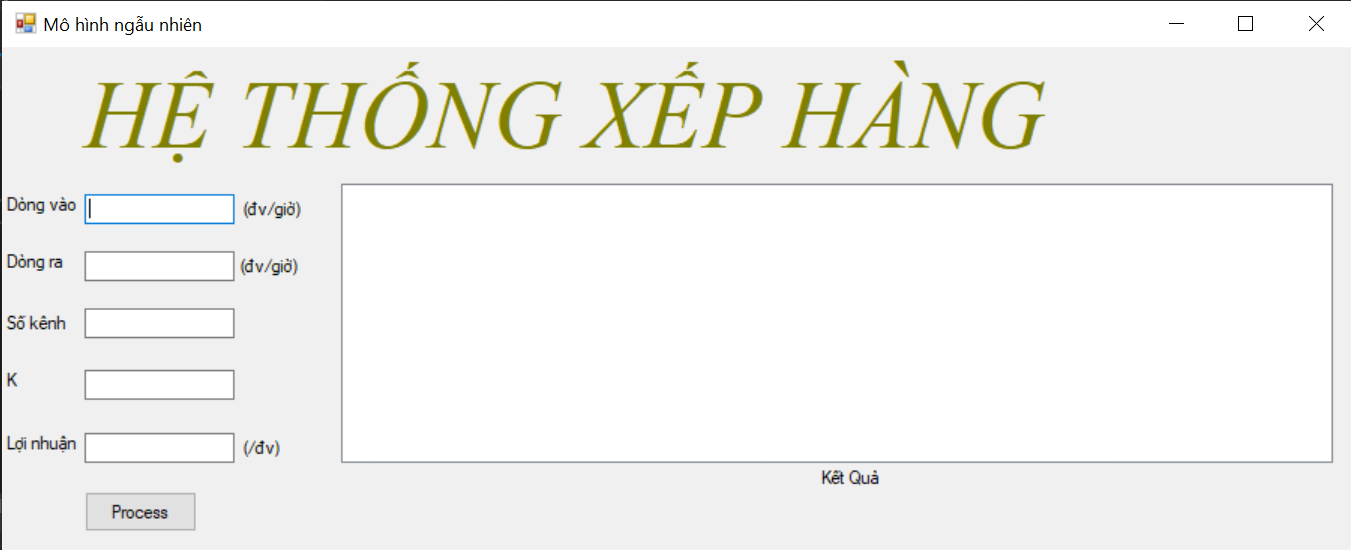
\includegraphics[scale=.5]{img/giaodien1.PNG}
    \end{center}
    \caption{Giao diện khi chưa input}
\end{center}

	
\end{block}
\end{frame}
%%%%%%%%%%%%%%%%%%%%%%%%%%%%%%%%%%%%%%%%%%%%%%%%%%%%%%%%%%%%%%%%%%%%%%%%%%%%%%%%%%%%%%%%%%%%%%%%%%%%%%%
\begin{frame}
	\frametitle{Áp dụng cho bài toán bán vé}
	\begin{block}{}
	\begin{center}
    \begin{center}
     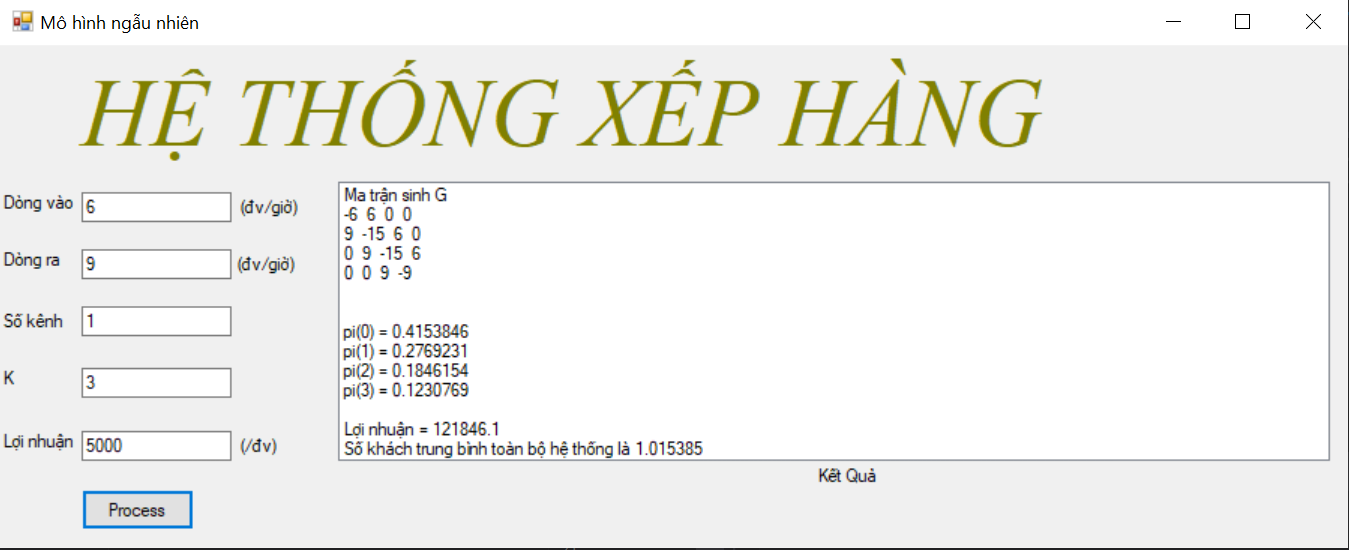
\includegraphics[scale=.5]{img/giaodien2.PNG}
    \end{center}
    \caption{Giao diện khi đã input}
\end{center}

	
\end{block}
\end{frame}
%%%%%%%%%%%%%%%%%%%%%%%%%%%%%%%%%%%%%%%%%%%%%%%%%%%%%%%%%%%%%%%%%%%%%%%%%%%%%%%%%%%%%%%%%%%%%%%%%%%%%%%%%%%%%%%%%%%%%%%%%%%%%%%%%%%%%%%%%
\end{document}